\section{Clase 19}
\subsection{Teorías de gauge}
Se divide en dos periodos:

\textbf{a) Periodo antiguo: 1918-1954}

\textbf{b) Periodo antiguo: 1954-actualidad}

La idea de gauge fue inspirada en la teoría general de la relatividad.

\subsubsection{Relatividad especial}

\begin{figure}[h!]
	\centering
	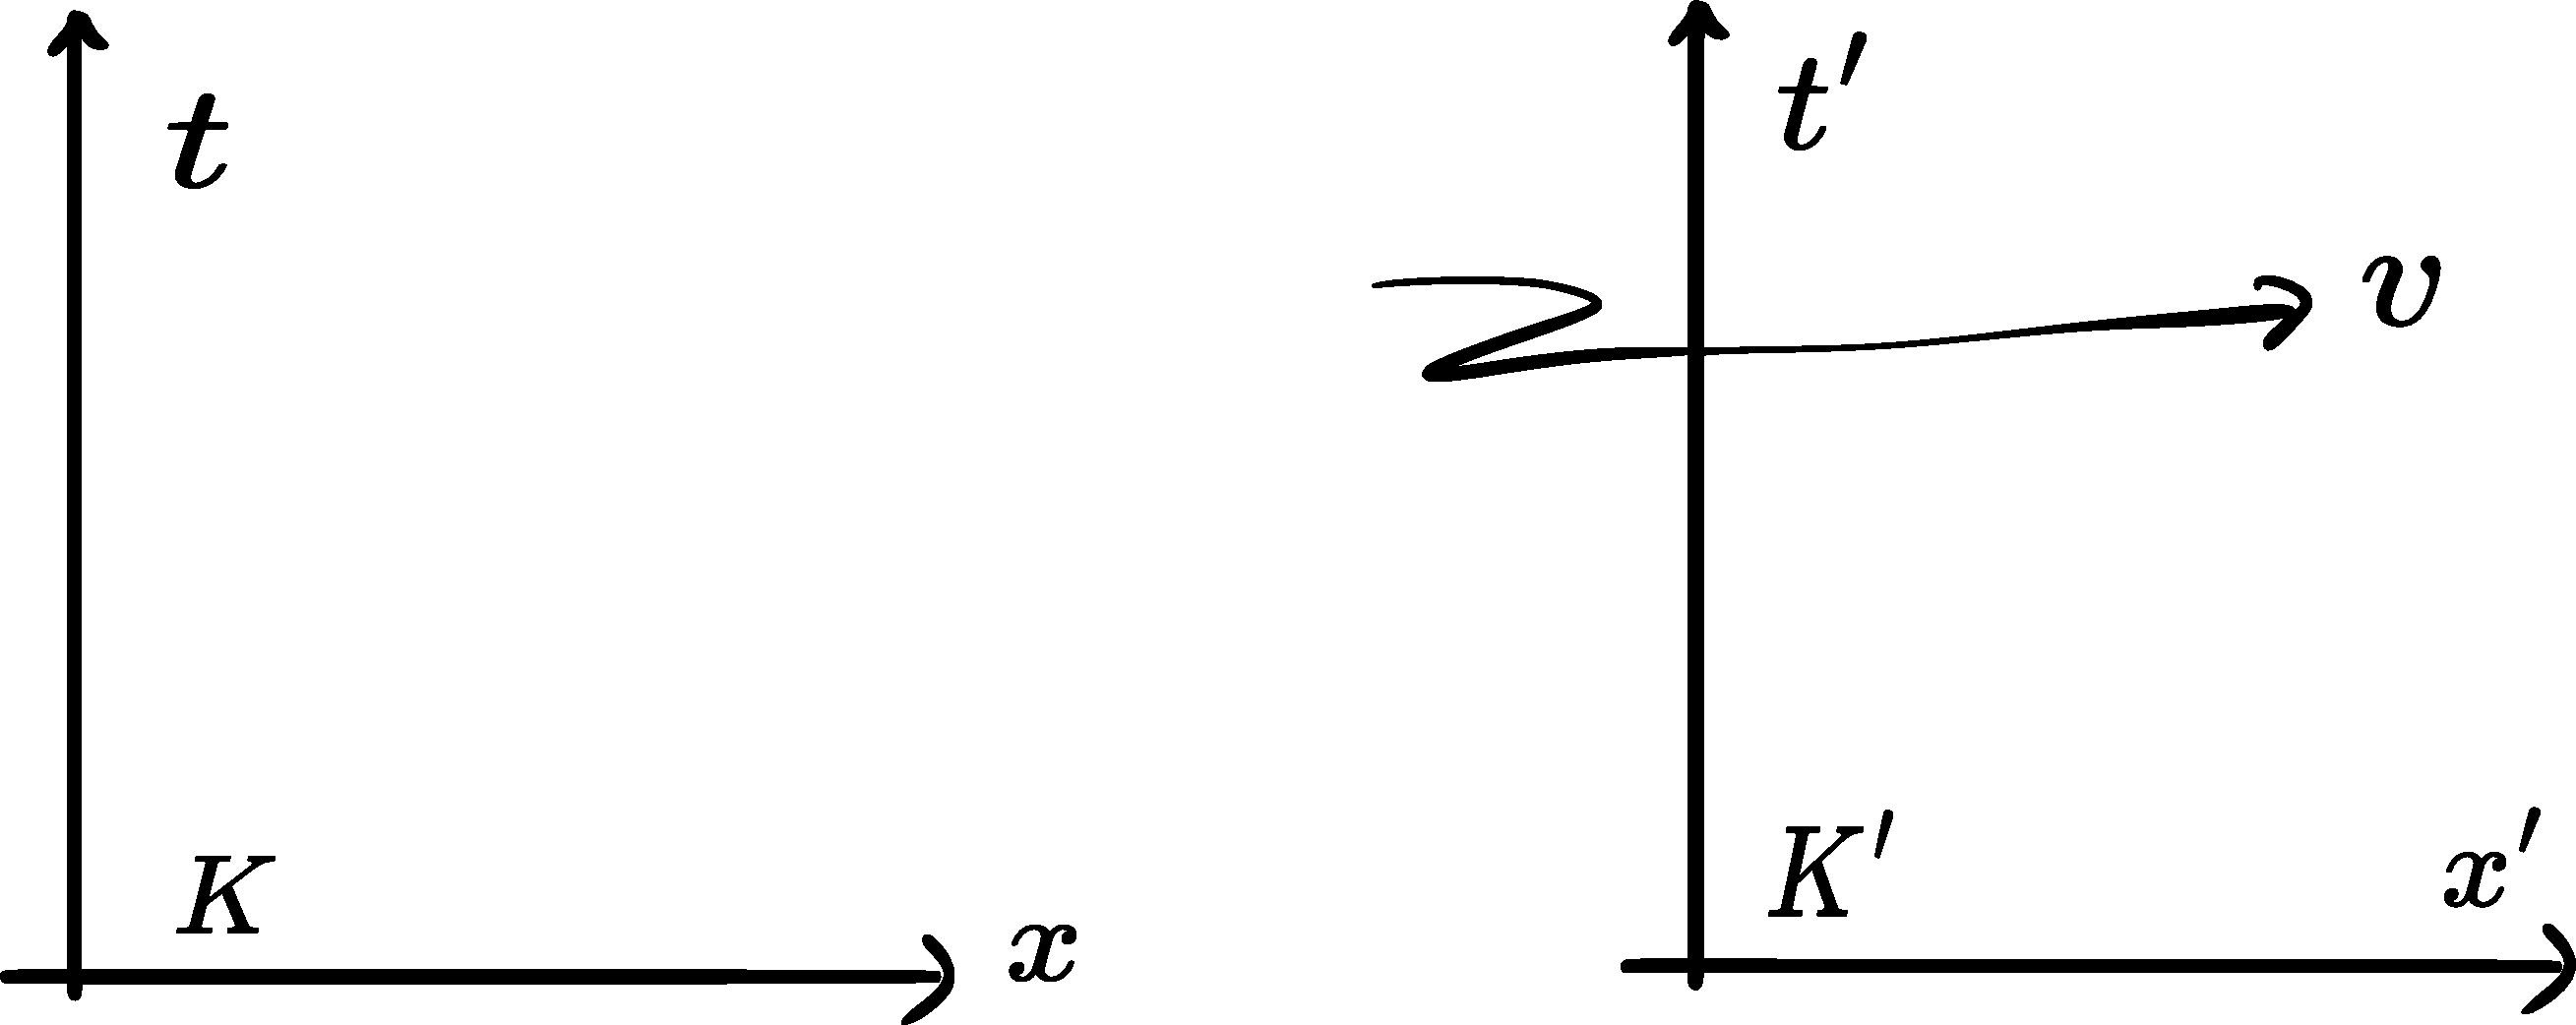
\includegraphics[scale=0.2]{fig/Galileo.pdf}
\end{figure}

¿Cómo se relacionan las medidas en el SRI $K$ con las hechas en el SRI $K'$? La respuesta es por medio de las transformaciones de Lorentz,
\begin{equation}
  x'^\m =\Lmn x^\n 
\end{equation}
que en una dimensión es dada por
\begin{align}
  x'^1&=\frac{x^1-\dfrac{v}{c}x^0}{\sqrt{1-v^2/c^2}}\\
  x'^0&=\frac{x^0-\dfrac{v}{c}x^1}{\sqrt{1-v^2/c^2}}
\end{align}

Estas transformaciones dependen solo de la velocidad entre los observadores, pero no dependen de la posición de dichos observadores. Esto implica que las transformaciones forman un grupo de parámetro constante $v/c$. \footnote{O desde el punto de vista de las rotaciones, $\tan\th =v/c$.} Luego, las transformaciones de Lorentz, son transformaciones globales.

\subsubsection{Relatividad general}
Consideremos un conjunto de observadores ubicados en ascensores que caen libremente sobre la Tierra. Estos observadores toman medidas de un fenómeno tal como el movimiento de una partícula en un campo gravitacional. 

%\textbf{IMAGEN}



\underline{\textit{Nota: }}Los símbolos de Christoffel miden el cambio en la dirección de un vector (o tensor) al ser transportado paralelamente

¿Cómo están relacionadas las medidas de estos observadores? Debido a que los diferentes SRI no se mueven uno con respecto al otro con velocidad constante, dichas medidas \textit{no} pueden estar relacionadas mediante una transformación de Lorentz. 

Las medidas de los observadores en los ascensores están conectadas por medio de \textit{transformaciones no-lineales},
\begin{equation}
  x'^\m =x'^\m (x^\n )
\end{equation}
o bien
\begin{equation}
  x'^\m =x^\m +\frac{1}{2}(\G ^\m _{\a\b })_Px^\a x^\b 
\end{equation}
con
\begin{equation}
  \G^\m _{\a\b }=\pdv{x'^\m }{x^\a }{x^\b }
\end{equation}

\subsection{Geometría de Weyl}
En la geometría de Riemann, un vector $\xi^\m $ que es trasladado paralelamente experimenta un cambio en su dirección, dado por
\begin{equation}
  \dd \xi^\m =\G^\m _{\a\b }\dd x^\a \xi^\b 
\end{equation}

En esta geometría, la dirección de un vector es un concepto relativo, ya que depende del SR, pero la longitud del vector, i.e.,  su norma, es constante, por lo cual, es un concepto absoluto.

Weyl consideró que la longitud del vector debería ser también un concepto relativo, es decir, que depende del observador. La norma de un vector es dada por
\begin{equation}
  l=(\xi^\m \xi_\m )^{1/2}
\end{equation}
Esto implica que si $g_{\m\n }$ es la métrica de la superficie, entonces
\begin{equation}\label{19.1}
  l^2=g_{\m\n }\xi^\m\xi^\n 
\end{equation}

Bajo traslación paralela, el largo $l$ del vector $\xi^\m $ cambia de acuerdo a
\begin{equation}\label{19.2}
  \dd l= \varphi_\b \dd x^\b l
\end{equation}
es decir, el cambio debe ser proporcional al largo $l$ y al desplazamiento $\dd x^\m $.

De \eqref{19.1} y \eqref{19.2} vemos que
\begin{align}
  \dd l^2&=\dd (g_{\a\b}\xi^\a \xi^\b )\\
  &=2l\dd l\\ 
  &=2l^2\varphi_\g \dd x^\g \\
  &=2 g_{\a\b }\xi^\a \xi^\b \varphi_\g \dd x^\g 
\end{align}
\begin{equation}\label{19.3}
\implies   \boxed{\dd l^2=2g_{\a\b }\varphi_\g \xi^\a \xi^\b \dd x^\g }
\end{equation}
Además,
\begin{align}
  \dd (g_{\a\b}\xi^\a \xi^\b )&=\partial_\g g_{\a\b }\dd x^\g \xi^\a \xi^\b +g_{\a\b }\dd \xi^\a \xi^\b +g_{\a\b }\xi^\a \dd\xi^\b \\
  &=\partial_\g g_{\a\b }\xi^\a \xi^\b \dd x^\g+g_{\a\b }\G^\a _{\m\n }\dd x^\m \xi^\n \xi^\b +g_{\a\b }\xi^\a \G^\b_{\m\n }\dd x^\m \xi^\n \\
  &=\left(\partial_\g g_{\a\b }+g_{\s \b }\G^\s_{\g\a }+g_{\a\s }\G^\s _{\g\b }\right)\xi^\a\xi^\b \dd x^\g \label{19.4}
\end{align}
donde hemos renombrado algunos índices de manera conveniente para poder factorizar. De \eqref{19.3} y \eqref{19.4} vemos
\begin{equation}\label{19.55}
  \partial_\g g_{\a\b }+g_{\s \b }\G^\s_{\g\a }+g_{\a\s }\G^\s _{\g\b }=2g_{\a\b }\varphi_\g 
\end{equation}
es decir,
\begin{equation}\label{19.5}
\boxed{  \nabla_\g g_{\a\b }=2g_{\a\b }\varphi_\g }
\end{equation}
o de manera equivalente
\begin{equation}
  \boxed{\nabla g=2 \varphi\otimes g,\qquad \varphi =\dd x^\m \varphi_\m }
\end{equation}

Notemos que si el lado derecho de \eqref{19.5} es igual a cero, recuperamos la condición de metricidad de la geometría de Riemann.

De \eqref{19.55} podemos despejar $\G^\a_{\b\g }$ usando ciclicidad, de donde se obtiene
\begin{equation}
  ^W\G ^\a_{\b\g }=\G^\a _{\b\g }+\d^\a_\b \varphi_\g +\d^\a_\g \varphi_\b -g_{\b\g }g^{\a\s }\varphi_\s 
\end{equation}
donde $\G^\a_{\b\g }$ son los símbolos de Christoffel usuales.

Consideremos de nuevo la ecuación \eqref{19.2}
\begin{equation}\label{19.2}
  \dd l= \varphi_\b \dd x^\b l
\end{equation}
Si llamamos $l_0$ al largo del vector en el punto $P$ y $l$ al largo del vector en el punto $Q$, luego,
\begin{align}
  \frac{\dd l}{l}&=\varphi_\b \dd x^\b \\
  \int_{l_0}^l\frac{\dd l}{l}&=\int_C\varphi_\b \dd x^\b \\
  \ln\left(\frac{l}{l_0}\right)&=\int_C\varphi_\b \dd x^\b \\
  l&=e^{\int_C\varphi_\b \dd x^\b }l_0
\end{align}
\begin{equation}\label{19.6}
  \implies \boxed{l^2=e^{2\int_C\varphi_\b \dd x^\b }l^2_0}
\end{equation}
Dado que $l^2=g_{\a\b }\xi^\a\xi^\b $ vemos que un cambio en la norma del vector generará un cambio en la métrica. Esto implica que si el largo del vector cambia punto a punto, entonces la métrica cambiará punto a punto. Entonces, la variedad $\mathcal{M}$ está dotada de una familia de métricas, una en cada punto. Para todas ellas se cumplirá que en un punto $x^\m $ se tiene
\begin{equation}\label{19.7}
  \nabla_\g g_{\a\b }=2g_{\a\b }\varphi_\g \Longleftrightarrow \nabla g=2\varphi\otimes g
\end{equation}
lo que implica que en otro punto $x^\m +\dd x^\m $ tenemos
\begin{align}\label{19.8}
  \nabla_\g \bar{g}_{\a\b }=2\bar{g}_{\a\b }\varphi_\g \Longleftrightarrow \nabla \bar{g}=2\varphi\otimes \bar{g}
\end{align}

Dado que en $x^\m $ tendríamos $l_0^2=g_{\m\n }\xi^\m\xi^\n $ y en $x^\m +\dd x^\m $ tendremos $l^2=\bar{g}_{\m\n }\xi^\m\xi^\n $. De \eqref{19.6},
\begin{align}
  \bar{g}_{\m\n }\xi^\m \xi^\n =e^{2\int_C\varphi_\b \dd x^\b }g_{\m\n }\xi^\m \xi^\n
\end{align}
\begin{equation}
  \implies \bar{g}_{\m\n } =e^{2\int_C\varphi_\b \dd x^\b }g_{\m\n }
\end{equation}
llamando 
\begin{equation}
  \chi =\int_C\varphi_\b \dd x^\b 
\end{equation}
tenemos
\begin{equation}\label{19.9}
\boxed{  \bar{g}_{\m\n}=e^{2\chi }g_{\m\n }} \Longleftrightarrow \bar{g}=e^{2\chi }g
\end{equation}
conocidas como las transformaciones de escala de Weyl o transformaciones conformes de la métrica. 

Para el lado izquerdo de \eqref{19.8}
\begin{align}
  \nabla\bar{g}&=\nabla(e^{2\chi }g)\\
  &=2\dd \chi e^{2\chi }g+e^{2\chi }\nabla g\\
  &=2\dd \chi \bar{g}+e^{2\chi }2\varphi g\\
  &=2\dd \chi \bar{g}+2\varphi \bar{g}\\
  &=2(\dd\chi +\varphi)\bar{g}
\end{align}
y el lado derecho de \eqref{19.8} nos dice que
\begin{equation}
  \nabla\bar{g}=2(\varphi +\dd\chi )\bar{g}=2\bar{\varphi}\bar{g}
\end{equation}
\begin{equation}
  \implies\boxed{ \bar{\varphi}=\varphi+\dd\chi}
\end{equation}
\begin{equation}
  \dd x^\m \bar{\varphi}_\m =\dd x^\m \varphi_\m +\dd x^\m \partial_\m \chi 
\end{equation}
\begin{equation}
  \implies \boxed{\bar{\varphi}_\m =\varphi_\m +\partial_\m \chi }
\end{equation}



















































